\subsection{Visualisierung der Klassifikation durch Annotationen}
    Eine wichtige Funktion des Systems und Bestandteil des Konzeptes
    ist die Visualisierung einer Klassifikation durch Annotationen
    auf der klassifizierten Webseite,
    weshalb an dieser eine Stelle die Ergebnisse
    für eine Klassifikation präsentiert werden.

    Abbildung \ref{image:findingTeachersAnnotationsOverview}
    zeigt Beispielhaft einen Ausschnitt der annotierten Übersichtsseite
    des Studienportals "`Babw"',
    welches Stellvertretend auch für die restlichen klassifizierten Portale
    steht\footnote{Die zu sehenden Darstellungsfehler oben rechts im Kopfbereich
    sowie am Anfang der Brotkrümelnavigation unter dem Portal
    sind der in Kapitel \ref{section:findingsMethod} beschriebenen
    Art und Weise der Einbindung des Annotator Plugins geschuldet.
    Durch die Zwischenschaltung der entwickelten Komponente
    führt der Browser Cross-Origin-Requests durch,
    um die genutzte Bibliothek für besondere Symbole zu beziehen.
    Diese Aufrufe werden allerdings unterbunden,
    weshalb die Symbole nicht korrekt dargestellt werden.
    Bei einer direkten Einbindung des Plugins wäre dies selbstverständlich nicht der Fall.
    Der fünfte Link im Kopfbereich wurde richtig klassifiziert.}.

    \begin{figure}[htb]
        \centering
        
\includegraphics[width=\textwidth]{../resources/findings/case-study-1/babw/annotations/overview.png}
        \caption{Annotierte Übersichtsseite der Lehrenden und Betreuenden im Portal BaBw}
        \label{image:findingTeachersAnnotationsOverview}
    \end{figure}

    Bis auf wenige Ausnahmen, die in unter anderem in
    Kapitel \ref{section:findingsTeachersAbnormalitiesBabw} besprochen werden,
    wurden alle klassifizierten Elemente korrekt hervorgehoben.

    Eine detaillierte Ansicht eine beispielhaften Annotation zeigt
    Abbildung \ref{image:findingTeachersSubjectAreaAnnotations}.

    \begin{figure}[htb]
        \centering
        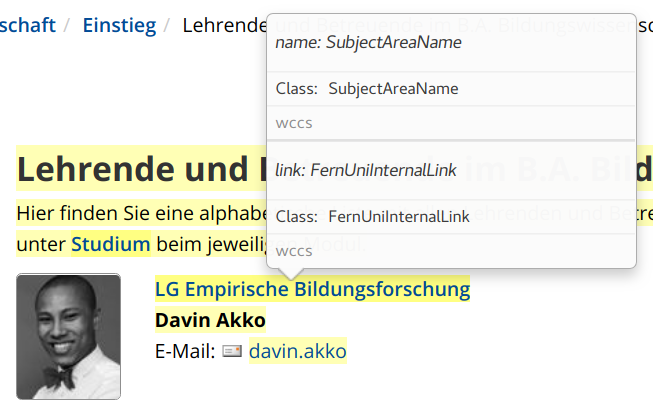
\includegraphics[scale=\screenshotScaleFactor]{../resources/findings/case-study-1/babw/annotations/double-lg-annotation.png}
        \caption{Annotationen eines Lehrgebietes}
        \label{image:findingTeachersSubjectAreaAnnotations}
    \end{figure}

    Das Lehrgebiet besitzt korrekterweise zwei Annotationen,
    da dieses Element sowohl den Namen als auch den Link enthält
    und deshalb doppelt klassifiziert wurde.